\uextra{Apéndice}{Resultados de la Validación de Usabilidad}
\label{apx:pruebas-usabilidad}

\begin{table}[H]
    \caption{Caracterización de los participantes}
    \label{tab:caracterizacion-participantes}
    \begin{tabularx}{\textwidth}{ l l l X }
        \hline
        \textbf{ID} & \textbf{Edad} & \textbf{Género} & \textbf{Experiencia previa en programación} \\
        \hline
        P01         & 13 años       & Femenino        & Scratch, MakeCode                           \\
        P02         & 16 años       & Masculino       & Scratch, Python                             \\
        P03         & 13 años       & Masculino       & Scratch                                     \\
        P04         & 10 años       & Masculino       & Ninguna                                     \\
        P05         & 10 años       & Masculino       & Scratch                                     \\
        \hline
    \end{tabularx}
\end{table}

\begin{table}[H]
    \caption{Resumen de resultados de las pruebas de usabilidad}
    \label{tab:resultados-usabilidad}
    \begingroup
    \renewcommand{\TableBodyFontSize}{\footnotesize}
    \setlength{\tabcolsep}{5pt}
    \begin{tabularx}{\textwidth}{l X X X X X X X}
        \hline
        \textbf{ID} & \textbf{Operaciones matemáticas} & \textbf{Manejo de textos} & \textbf{Operaciones lógicas} & \textbf{Control de flujo} & \textbf{Uso de listas} & \textbf{Uso de micro:bit} & \textbf{Desafíos de su nivel} \\
        \hline
        P01         & Sin ayuda                        & Sin ayuda                 & Con ayuda                    & Con ayuda                 & Sin ayuda              & Sin ayuda                 & Con ayuda                     \\
        P02         & Sin ayuda                        & Sin ayuda                 & Sin ayuda                    & Sin ayuda                 & Con ayuda              & Sin ayuda                 & Sin ayuda                     \\
        P03         & Sin ayuda                        & Con ayuda                 & Sin ayuda                    & Con ayuda                 & Con ayuda              & Sin ayuda                 & Con ayuda                     \\
        P04         & Con ayuda                        & Con ayuda                 & Con ayuda                    & Con ayuda                 & Con ayuda              & Con ayuda                 & Con ayuda                     \\
        P05         & Sin ayuda                        & Con ayuda                 & Sin ayuda                    & Con ayuda                 & Con ayuda              & Con ayuda                 & Con ayuda                     \\
        \hline
    \end{tabularx}
    \endgroup
\end{table}

\begin{figure}[H]
    \label{fig:pruebas-usabilidad-p1}
    \centering
    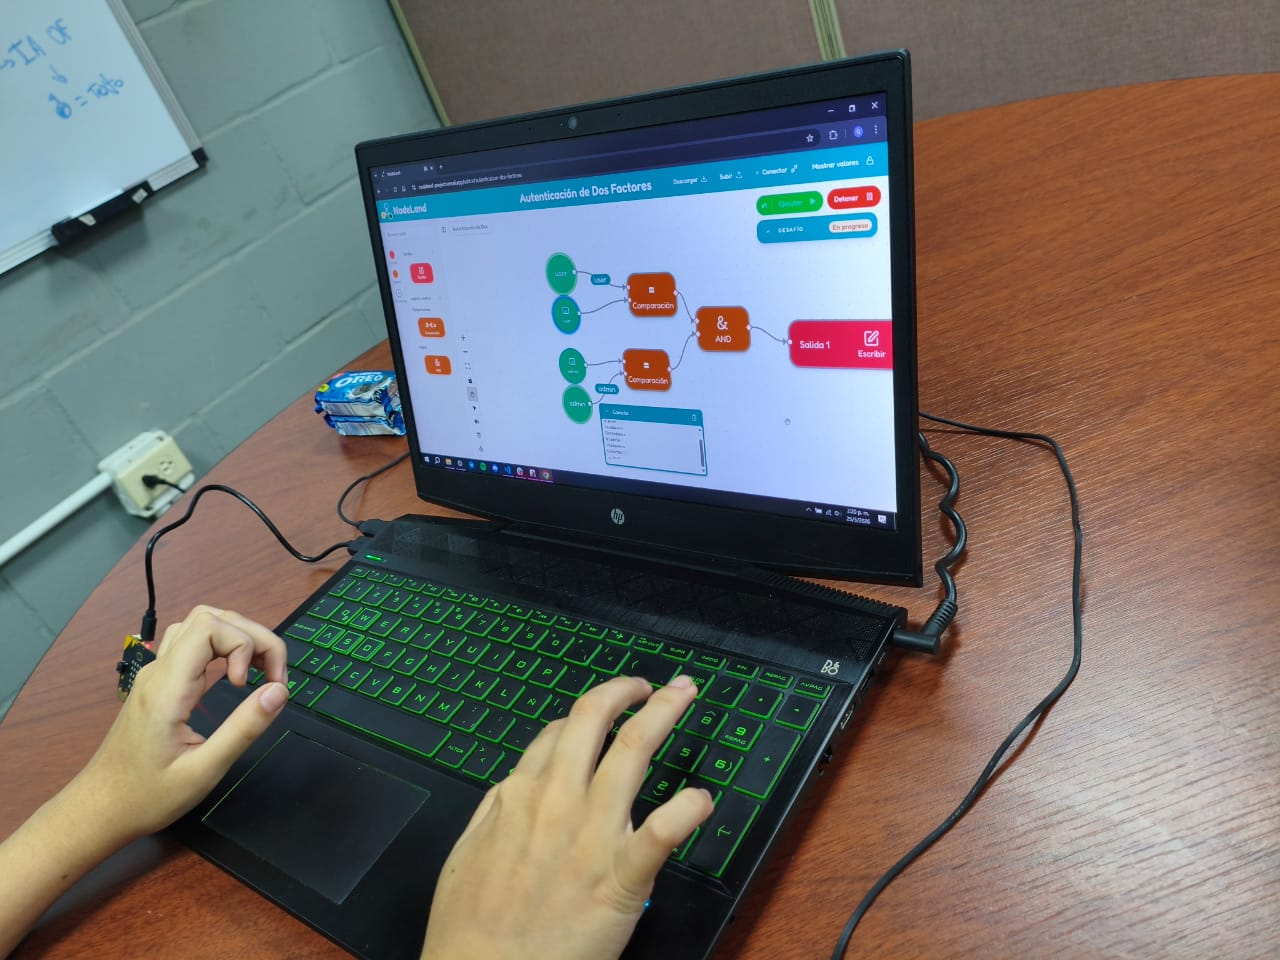
\includegraphics[width=0.7\textwidth]{images/validation/validation-1.png}
    \caption[Pruebas de usabilidad con estudiante P01]{Pruebas de usabilidad con estudiante P01}
\end{figure}